\chapter{通信高效的分布式优化算法}
\author{Gauri Joshi and Shiqiang Wang}

\section*{摘要}
在联邦学习中,连接边缘参与者和中央聚合器的通信链路有时是有带宽限制的,而且会有很高的网络延迟。因此,设计和部署具有通信高效的分布式训练算法是急需的。在本章中,我们将回顾两种不同的具有通信高效的分布式随机梯度下降(SGD)方法:(1)本地更新随机梯度下降(SGD),客户端进行多次本地模型更新,并周期性的进行聚合;(2)梯度压缩和稀疏化方法,以减少每次更新传输的比特数。在这两种方法中,误差收敛与迭代次数和通信效率之间存在着权衡关系。

\section{引言}

\textbf{ML训练中的随机梯度下降。}大多数监督学习问题都是使用经验风险最小化框架来解决的\cite{boyd2004convex, shalev2014understanding},其目标是最小化经验风险目标函数$F(\bm{x}) = \sum_{j=1}^{n} f(\bm{x}, \xi) / n$。其中,$n$是训练数据集的大小,$\xi_{j}$是第$j$个已标注的训练样本,$f(\bm{x},\xi_{n})$是(通常是非凸的)损失函数。一种普遍优化$F(\bm{x})$的算法是随机梯度下降(SGD)。在这种算法中,我们计算$f(\bm{x},\xi_{n})$在小的、随机选择的子集$\mathcal{B}$(称为迷你批次)上的梯度,每个子集有$b$个样本\cite{bottou2018optimization, dekel2012optimal, li2014efficient, robbins1951stochastic, ruder2016overview, pmlr-v84-yin18a},并根据$\bm{x}_{k+1} = \bm{x}_{k} - \eta \sum_{i \in \mathcal{B}} \nabla f(\bm{x}_{k};\xi_{i})/b$ 更新$\bm{x}$,其中$\eta$被称为学习率或步长。虽然算法是为凸目标设计的,但由于小型批量SGD有能力摆脱鞍点和局部最小值\cite{chaudhari2018stochastic, neyshabur2017geometry, shwartzziv2017opening, zhang2021understanding},因此即使在非凸损失表面也有良好的表现。因此,它是最先进的机器学习中的主导训练算法。

对于像Imagenet\cite{russakovsky2015imagenet}这样的大规模数据集,在单个节点上运行小批量的SGD可能会非常慢。进行梯度计算并行化的一个标准方法是参数服务器(PS)框架\cite{dean2012large},由一个中央服务器和多个工作节点组成。拖拽的工人节点和通信延迟会成为将这个框架扩展到大量工人节点的瓶颈。一些方法,如异步\cite{cui2014exploiting, dutta2018slow, gupta2016model, zhang2017yellowfin}和周期性梯度聚合\cite{stich2018local, wang2019cooperative, yu2019parallel}已被提出,以提高基于数据中心的ML训练的可扩展性。

\textbf{联邦学习的动机。}尽管算法和系统的进步提高了效率和可扩展性,但基于数据中心的训练仍有一个主要局限。它要求将训练数据集集中在参数服务器上,由它在工作节点上进行打乱和拆分。手机、物联网传感器和具有设备上计算能力的相机等边缘方的迅速扩散,导致了这种数据分区模式的重大转变。边缘方从它们的环境中收集丰富的信息,这些信息可用于数据驱动的决策。由于有限的通信能力以及隐私问题,这些数据不能直接发送到云端进行集中处理或与其他节点共享。联邦学习框架建议将数据留在边缘方,而将模型训练放在边缘。在联邦学习中,数据被保存在边缘方,模型以分布式的方式被训练。只有梯度或模型更新在边缘方和聚合器之间进行交换。

\begin{figure}[h]
	\centering
	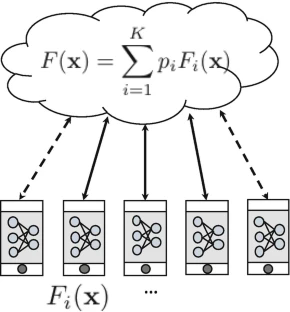
\includegraphics{images/chap06/Fig1}
	\caption{在联邦优化中,聚合器的目标是最小化边缘方局部目标函数$F_{i}(\bm{x})$的加权平均值}
	\label{fig:6.1}
\end{figure}

\textbf{系统模型和符号。}如图\ref{fig:6.1}所示,一个典型的联邦学习设置包括一个连接到$K$个边缘方的中央聚合器,其中$K$可能是数千甚至数百万的量级。每一方$i$都有一个由$n_{i}$个样本组成的本地数据集$\mathcal{D}_{i}$,它不能被传输到中央聚合器或与其他边缘方共享。我们用$p_{i} = n_{i}/n$来表示第$i$方所占数据比例,其中$n=\sum_{i=1}^{K}n_{i}$。聚合器试图用本地数据集的并集$\mathcal{D} = \cup_{i=1}^{K}\mathcal{D}_{i}$来训练一个机器学习模型$\bm{x} \in \mathbb{R}^{d}$。模型向量$x$包含模型的参数,例如,神经网络的权重和偏差。为了训练模型$x$,聚合器试图最小化以下经验风险目标函数:
\begin{align}
	F(\bm{x}) := \sum_{i=1}^{K}p_{i}F_{i}(\bm{x})
\end{align}
其中$F_{i}(\bm{x}) = \frac{1}{n_{i}}\sum_{\xi \in \mathcal{D}_{i}} f(\bm{x};\xi)$是第$i$方的本地目标函数。$f$是由模型$\bm{x}$定义的损失函数(可能是非凸的),$\xi$代表本地数据集$\mathcal{D}_{i}$的一个数据样本。请注意,我们分配的权重与第$i$方的数据比例成正比。这是因为我们想模拟一个集中式的训练场景,将所有的训练数据传输到一个中央参数服务器。因此,拥有更多数据的一方将在全局目标函数中获得更高的权重。

由于边缘方的资源限制和大量参与方,联邦训练算法必须在严格的通信限制下运行,并应对数据和计算的异质性。例如,连接每个边缘方和中央聚合器的无线通信链路可能有带宽限制,并且有很高的网络延时。另外,由于网络连接有限和电池的限制,边缘方可能只是间歇性地可用。因此,在给定的时间内,只有$K$个边缘方中只有$m$个子集可以参与训练模型$x$。为了在这些通信约束条件下运行,联邦学习框架需要新的分布式训练算法,超越在数据中心环境中使用的算法。在第6.2节中,我们回顾了local-update SGD算法及其变体,这些算法减少了边缘各方与聚合器的通信频率。在第6.3节中,我们回顾了压缩和量化的分布式训练算法,这些算法减少了边缘各方发送给聚合器的每次更新的比特数量。

\section{Local-Update SGD和FedAvg}

在本节中,我们首先讨论local-update SGD及其变体。FedAvg算法是联邦学习的核心,它是local-update SGD的扩展。我们将讨论FedAvg如何建立在local-update SGD之上,以及在联邦学习中用来处理数据和计算异质性的各种策略。

\subsection{Local-Update SGD及其变体}

\textbf{同步分布式SGD。}在数据中心的设置中,训练数据集$\mathcal{D}$被打乱并平均分配到$m$个工作者节点中。训练机器学习模型的标准方法是使用同步分布式SGD,其中梯度由工作者节点计算,然后由中央参数服务器汇总。在同步SGD的第t次迭代中,工作者从参数服务器中拉取模型的最新版本$x_{t}$。每个工作者$i$使用从本地数据集$\mathcal{D}_{i}$中抽取的B个样本的小批量数据$\mathcal{B}$来计算一个小批量随机梯度$g_{i}(x) = \sum_{\xi \in \mathcal{B}} f(x;\xi)$。然后,参数服务器收集来自所有工作者的梯度,并按以下方式更新模型参数
\begin{align}
	\bm{x}_{t+1} = \bm{x}_{t} - \frac{\eta}{m}\sum_{i=1}^{m}g_{i}(\bm{x})
\end{align}
随着工作者数量$m$的增加,同步SGD的误差与迭代收敛性得到改善。然而,由于工作者的局部梯度计算时间存在差异,等待所有工作者完成梯度计算的时间也会增加。为了提高工作者数量的可扩展性,中提出了同步SGD的<mark>拖拽者弹性变体</mark>,进行异步梯度聚合。

\textbf{Local-Update SGD。}尽管异步聚合方法对提高分布式SGD的可扩展性很有效,但在许多分布式系统中,工作者和参数服务器之间交换梯度和模型更新的通信时间会主导本地梯度计算时间的变化。因此,每次迭代后的节点间的持续通信可能是过于昂贵和缓慢的。Local-Update SGD是一种通信效率高的分布式SGD算法,它通过让工作者节点执行多次本地SGD更新而不是仅仅计算一个小批量梯度来克服这个问题。

如图6.2所示,Local-Update SGD将训练分为几轮通信。在一个通信轮中,每个工作者使用SGD对其目标函数$F_{i}(x)$进行局部优化。每个工作者$i$从当前的全局模型开始,用$x_{t}$表示,并执行$\tau$次SGD迭代,以获得模型$x_{t+\tau}^{(i)}$。然后,所得到的模型由$m$个工作者发送到参数服务器,服务器对其进行平均,以更新全局模型,如下所示:

$$
x_{t+\tau} = \frac{1}{m}\sum_{i=1}^{m}x_{t+\tau}^{(i)}。
$$

\textbf{Local-Update SGD每一次迭代的运行时间。}通过在与参数服务器通信之前在每个工作器上执行τ个本地更新,本地更新SGD减少了每次迭代的预期运行时间。让我们通过考虑以下延迟模型来量化这种运行时间的节省。第i个工作者在第k个局部步骤计算小批梯度的时间被建模为随机变量Yi,k∼FY,假定在工作者和小批之间是独立和相同的分布(i.i.d)。通信延迟用一个常数D表示,它包括将本地模型发送到参数服务器和从参数服务器接收平均的全局模型所需的时间。由于每个工人i进行了τ次本地更新,其平均本地计算时间(完成图6.3中3个蓝色箭头的一个序列所需的时间)由以下公式给出
$$\bar{Y} = \frac{Y_{i, 1} + Y_{i, 2} + \cdots + Y_{i, \tau}}{\tau}$$
如果τ=1,在这种情况下,本地更新SGD会简化为同步SGD,那么随机变量Y与Y是相同的。
$$
\mathbb{E}[T_{Local-update}] = \mathbb{E}[max(\bar{Y}_{1}, \bar{Y}_{1}, \cdots, \bar{Y}_{m}] + \frac{D}{\tau} \\
= \mathbb{E}[\bar{Y}_{m:m}] + \frac{D}{\tau}
$$
术语$Y_{m:m}$表示具有概率分布$Y \sim F_{Y}$的$m$个i.i.d.随机变量的最大顺序统计。从(6.6)中我们可以看出,执行更多的局部更新可以通过两种方式减少每次迭代的运行时间。首先,通信延迟在τ次迭代中得到摊销,并减少了一个系数τ。其次,执行局部更新也提供了一个减少散兵游勇的好处,因为$\bar{Y}_{m:m}$的尾部比$Y_{m:m}$轻,因此(6.6)中的第一个项随着$\tau$而减少。

**本地更新SGD的错误收敛**。正如我们在上面看到的,将工作者和参数服务器之间的通信频率降低到在τ迭代中只有一次,可以使每次迭代的运行时间大大减少。然而,设定一个大的$\tau$值,局部更新的数量会导致较差的误差收敛。这是因为,随着$\tau$的增加,工作节点的模型$x^{(i)}_{t+\tau}$会相互偏离。论文给出了局部更新SGD在局部更新数量$\tau$方面的错误收敛分析。假设目标函数$F(x)$是$L$-Lipschitz光滑的,学习率$\eta$满足$\eta L + \eta^{2}L^{2}\tau(\tau - 1) ≤ 1$。随机梯度$g(x; \xi)$是$\nabla F(x)$的无偏估计,即$\mathbb{E}_{\xi}[g(x; \xi)] = \nabla F(x)$。随机梯度$g(x; \xi)$被假定为有边界的方差,即$Var(g(x; \xi))≤\sigma^{2}$。如果起点是$x_{1}$,那么经过局部更新SGD的$T$次迭代后,$F(x_{T})$被约束为
$$
\mathbb{E}[\frac{1}{T}\sum_{t=1}^{T}\|\nabla F(x_{t})\|^{2}] \leq \frac{2[F(x_{1}-F_{\inf})]}{\eta t} + \frac{\eta L \sigma^{2}}{m} + \eta^{2}L^{2}\sigma^{2}(\tau - 1)
$$
其中$x_{t}$表示第$t$次迭代时的平均模型。设置$\tau=1$使得本地更新SGD及其误差收敛边界与同步分布式SGD相同。随着$\tau$的增加,约束的最后一项会增加,从而增加收敛时的误差底线。

**适应性沟通策略**。从上面的运行时间和误差分析中,我们可以看到,当我们改变τ时,每个迭代的误差和通信延迟之间存在着权衡。 较大的$\tau$可以减少预期的通信延迟,但是产生更差的误差收敛。为了获得快速收敛和低误差底线,提出了一个在训练过程中适应$\tau$的策略。对于一个固定的学习率$n$,中的以下策略会逐渐减少$\tau$:
$$
\tau_{\ell} = \left \lceil \sqrt{\frac{F(x_{t=\ell T_{0}})}{F(x_{t=0})}}\tau_{0} \right \rceil
$$
其中,$\tau_{\ell}$是训练中$T_{0}$秒的第$\ell$个区间内的局部更新次数。这个更新规则也可以被修改,以考虑到基本的可变学习率时间表(图6.4)。

**弹性平均法和重叠SGD**。在本地更新的SGD中,在下一组τ更新开始之前,需要将更新的全局模型传达给各节点。此外,在m个节点中最慢的节点完成其τ个本地更新之前,全局模型不能被更新。这种通信障碍会成为全局模型更新的瓶颈,并增加每轮训练的预期运行时间。由于这种通信障碍是由算法而不是系统实现强加的,我们需要一种算法方法来消除它,并允许通信与本地计算重叠。诸如等作品使用异步梯度聚合来消除同步障碍。然而,异步聚合会导致模型僵化,也就是说,慢速节点会有任意过时的全局模型版本。最近的一些工作提出了本地更新SGD的变种,允许通信和计算的重叠。在这些算法中,工作节点从一个锚模型开始他们的本地更新,该模型甚至在最慢的节点完成上一轮本地更新之前就可以使用。这种方法受到提出的弹性平均SGD(EASGD)算法的启发,该算法在目标函数中增加了一个近似项。近似方法,如,虽然不是为此目的而设计的,但自然允许通信和计算的重叠。

6.2.2 联合平均法(FedAvg)算法及其变体

**FedAvg算法。**由于在联合学习中,边缘伙伴的通信能力有限,本地更新的SGD特别适合于联合学习的132G。Joshi和S. Wang的学习框架,在这里它被称为FedAvg算法。其主要区别如下。首先,作为云中服务器的工作节点被移动和物联网设备等边缘方所取代。由于边缘方的间歇性可用性,与数据中心的设置不同,每轮训练中只有K方中的m个子集参与。其次,数据集Dican的大小和组成在边缘方之间都是高度异质的,不像数据中心的设置,数据集D被洗牌并均匀地划分到工人节点。

联合平均算法(FedAvg)也将训练分为通信轮。在一个通信轮中,聚合器从可用的各方中均匀地随机选择m个边缘方。每个边缘方使用类似于局部更新SGD的SGD对其目标函数Fi(x)进行局部优化。与基本的本地更新SGD不同的是,每个工作者执行相同数量的本地更新τ,在FedAvg中,本地更新的数量τ可能在不同的边缘方和通信回合中有所不同。一个常见的实施做法是,各方运行的本地纪元E是相同的。因此,τi= �Eni其中B是小批量的大小。另外,如果每个通信轮次在壁钟时间上有一个固定的长度,那么τirep代表i方在时间窗口内完成的局部迭代,并且可能在不同的客户(取决于他们的计算速度和可用性)和不同的通信轮次中变化。在第r轮通信中,边缘各方从全局模型xr,0开始,各自进行τi个局部更新。假设他们得到的模型用x(i) r,τi表示。共享的全局模型xris的更新方式如下。
其中pi=|Di||D|,第i个边缘方的数据部分。

**处理数据异质性的策略。**由于数据集在各节点间高度异质化,边缘方的本地训练模型可能彼此有很大的不同。而且随着本地更新数量的增加,模型可能会变得对本地数据集过度拟合。因此,FedAvg算法可能会收敛到一个不正确的点,而这个点不是全局目标函数F(x)的静止点。例如,假设每个边缘方执行了大量的局部更新,第i方的局部模型收敛到x(i)∗= min Fi(x)。那么这些局部模型的加权平均将收敛于x=�Ki=1pix(i)∗,这可能与真正的全局最小值x∗=min F(x)有任意的不同。为了减少这种由数据异质性引起的求解偏差,一个解决方案是选择一个小的或衰减的学习率η和或保持小的局部更新数量τ。其他用于克服解决方案偏差的技术包括近似的局部更新方法,如,该方法为全局目标添加了一个正则化项,以及旨在最小化跨方模型的方法。通过交换控制变量来实现漂移。在高层次上,这些技术阻止了边缘方的模型偏离全局模型的情况。

**处理计算异质性的策略**数据异质性的影响会因边缘各方的计算异质性而加剧。即使边缘各方进行不同数量的局部更新τi,标准的FedAvg算法建议将所产生的模型按照数据比例pi进行简单的聚合。然而,这可能会导致一个不一致的解决方案,与预期的全局目标不匹配,如所示,并在图6.5中说明。最终的解决方案变得偏向于局部最优x(i)∗= min Fi(x),而且它可能离全局最小x(i)∗= min F(x)有任意的距离。论文通过将累积的局部更新(x(i)r,τi- x(i)r,0)按局部更新的数量τi进行归一化,然后再将其发送到中央聚合器,从而解决了这种不一致的情况。这种被称为FedNova的规范化联合平均算法的结果是一致的解决方案,同时保留了快速收敛率。

除了局部更新数量τi的变化,由于边缘方使用局部动量、自适应局部优化器(如AdaGrad)或不同的学习率计划,也可能出现计算异质性和解决方案不一致的情况。在这些情况下,需要一个通用的FedNova版本来解决不一致的问题。

**处理边缘方间歇性可用性的策略** 在一个联合学习设置中,边缘方的总数可以达到数千甚至数百万台设备的数量。由于本地计算资源的限制和带宽的限制,边缘方只能间歇性地参与训练。例如,目前手机只有在插电充电时才会被用于联合训练,以节省电池。因此,在每一轮通信中,只有一小部分边缘方参与到FedAvg算法中。大多数关于设计和分析联合学习算法的工作都假设边缘方的子集是从整个边缘方集合中均匀地随机选择的。这种部分和间歇性的参与通过给误差增加一个方差项而放大了数据异质性的不利影响。最近一些134G. Joshi和S. Wang的作品提出了应对这种异质性并提高收敛速度的客户端选择方法。这些策略将更高的选择概率分配给具有较高局部损失的边缘方,并表明它可以加速全局模型的进展。然而,这种加速是以较高的非消失偏差为代价的,这种偏差随着数据异质性程度的增加而增加。论文提出了一种自适应策略,逐渐减少选择倾斜,以实现收敛速度和误差底限之间的最佳权衡。

模型压缩

除了执行多个本地更新外,模型在通信和计算过程中也可以被压缩。一种方法是使用标准的无损压缩技术,然而,这只能在有限的程度上减少模型的大小,并且需要在接收方进行解压。在本节中,我们将讨论一类特殊的有损压缩技术,该技术旨在提高联合学习和分布式SGD中的通信效率。这些技术不需要在接收方进行解压缩,并且可以保证训练收敛。我们在第6.3.1和6.3.2节中重点讨论了提高通信效率的方法。6.3.1和6.3.2节中重点介绍了提高通信效率的方法,在6.3.3节中重点介绍了提高通信和计算效率的方法。

有压缩更新的SGD

一个广泛使用的方法是压缩各方和聚合器之间传输的模型更新。特别是,我们定义了一个压缩器C(z),它产生任意向量z的压缩版本。流行的压缩器包括那些实现量化和稀疏化的压缩器。根据它们的特点,压缩机可以分为无偏和一般(即可能有偏)。我们在下文中讨论这两种压缩机的变体,其中我们考虑了一种叫做一般压缩机的误差反馈技术,这种技术对于避免方差爆炸和保证收敛是很有用的。请注意,我们在本节中的偏见概念是在概率建模的背景下,无偏见的压缩机意味着压缩向量的期望值(从该压缩机得到)等于原始向量。

没有误差反馈的无偏压制器

一个无偏的压缩器C(z)满足以下两个特征。
其中,q≥0是一个常数,用于捕获压缩机实现的相对近似差距。直观地说,相对逼近差距意味着压缩后的向量与原始向量相比的相对误差。我们很容易看到,q=0是C(z)=z(即不压缩)的必要条件,q=1是C(z)=0(即不传输)的必要条件。一般来说,较大的q对应于由C(z)产生的更多的压缩矢量。正如我们在接下来介绍的 "随机-k "例子中所看到的,在某些情况下,我们可能会放大压缩结果以保证无偏性,这可能会产生一个大于1的q值。

例子 无偏差压缩器的一个例子是一个随机量化器,它给出了
为该向量的第i个分量,其中�-�和�-�分别表示底限(向下舍入为整数)和上限(向上舍入为整数)运算符。我们注意到,在浮点表示法的情况下,这里的整数可以是基数。可以很容易地看出,这种量化操作满足无偏性属性(6.10)。注意到量化操作给出q = maxy∈[0,1](1-y)2y + y2(1-y),我们有q = 1

另一个例子是,从原始向量z中随机选择k个分量,其概率相同为k
为矢量的第i个分量。这通常被称为随机-k稀疏化技术。显然,这种操作也是无偏的。(6.11)的左手边是�(d)的总和。

**带有压缩更新的本地更新SGD。**当使用压缩和本地更新SGD时,每一方都像往常一样计算其本地更新。这些更新在发送到聚合器之前被压缩,然后聚合器对压缩的更新进行平均,以获得下一个全局模型参数。假设一个有τ个迭代的回合从迭代t开始,这就给出了以下递推关系。

在不同的实现中,可以在服务器上应用另一种压缩操作,以保持相同的压缩水平(例如,量化精度或要传输的组件数量)。这样就可以得到

(6.14)和(6.15)中的操作是相似的,可能是整体近似间隙q不同。

**收敛的边界。**在适当选择学习率的情况下,使用(6.14)进行T次迭代后的最优性(以梯度的平方准则表示)可以被约束为。
其中xt:=1m�mi=1x(i)t对于所有t,即使没有压缩

**差异化吹捧。**从(6.16)中,我们可以看到,当T足够大时,误差由第一项O�1+q√T�主导。当q很大时,我们需要将迭代次数T增加q2倍才能消除q的影响并达到相同的误差,这是有问题的,因为压缩的优势会被增加的计算量所抵消,特别是对于随机-k这样的压缩器,1+q与k成反比,正如我们前面讨论的那样。由于(6.16)的第一项也与随机梯度的方差成正比,为了简单起见,我们将其吸收到O(-)的符号中,这种现象在文献中也被称为方差吹胀。

接下来,我们将看到,误差反馈可以通过在本地积累压缩参数向量和实际参数向量之间的差异来解决方差吹大的问题,这样就可以在未来的通信回合中传输。

 带有误差反馈的普通压缩机

我们首先介绍一个一般的(可能是有偏见的)压缩器。一般的压缩器C(z)满足以下属性。

其中,α是一个常数,0≤α<1,表示压缩机实现的相对近似差距。与(6.10)和(6.11)中无偏压缩器的特性相比,关键的区别是一般压缩器不保证无偏性。当我们让α=q时,方程(6.11)和(6.17)基本上是相同的,只是为了收敛分析的目的,我们要求α<1。保持α与q不同的另一个原因是为了区分两种类型的压缩机。满足(6.17)的压缩机也被称为α-收缩性压缩机。还有一个更严格的(6.17)版本,其中不等式在没有期望的情况下成立。

例子 一般压缩器的一个典型例子是top-k稀疏化技术,它选择幅度最大的k个分量。这可以表示为:。

为矢量的第i个分量。由于这个操作对给定的z来说是确定的,所以它是有偏差的。我们可以得到α=1-kdb,因为z中其余分量的平方不能大于幅度最大的k个分量。

**具有压缩更新和错误反馈的本地更新SGD。**当使用错误反馈时,除了在客户端和服务器之间交换压缩的更新外,未被传达的部分(这里称为 "错误")将在本地累积。在下一轮中,累积的误差将被添加到该轮的最新更新中,这个和向量将被压缩器用来计算压缩向量。每一方i保留一个误差向量e(i),初始化为e(i)0=0。 在每一轮r中,执行以下步骤。

1. 对于每一方i∈{1, 2, . . . a. 从全局参数xr开始,计算局部梯度下降的τ步,以获得x(i) r,τ。
	b. 将累积误差与当前更新相加:z(i)r:= e(i)r+x(i)r,τ-xr。
	c. 计算压缩结果�(i)r:= C�z(i)r�(这就是将被发送给聚合器的结果)。
	d. 减去压缩结果,得到下一轮的剩余误差 e(i) r+1= z(i)r- �(i)r。
	
	2. 聚合器根据从各方收到的压缩更新来更新下一轮的全局参数,即138G. Joshi和S. Wang xr+1= xr+ 1 m m� i=1�(i)r= xr+ 1 m m� i=1 C�z(i)r�。(6.19) 我们可以看到(6.14)和(6.19)的唯一区别是,我们现在对z(i)r进行压缩,这包括前几轮的累积误差。注意,为了方便起见,我们在这里使用r轮索引,而不是(6.14)中的迭代索引t。与(6.15)类似,上述程序也可以扩展到压缩和累积双方和聚合器的误差。
	
	**收敛的边界。**与(6.16)类似,我们提出错误反馈机制的最优性约束。在适当选择学习率的情况下,我们有
	我们注意到,尽管(6.16)和(6.20)的左手边略有不同,但它们的物理含义是相同的。这种微小的差异是由于在推导这些界限时使用了不同的技术。与(6.16)相比,我们看到由于压缩而产生的近似差距,由α捕获,现在在(6.20)的第二项中。当T足够大时,我们现在的收敛率为O�1√T�,这就避免了方差爆炸的问题。
	
	请注意,由于我们要求0≤α<1,我们这里的分析对(6.13)中的随机-k压缩器不成立。(6.13)中的随机-k压缩器,但我们可以修改(6.13),去掉放大系数d/k,因为我们不再要求无偏性了。所得的得到的压缩器满足α=1-k/d,这与top-k的压缩器相同。然而,在实践中,top-k通常比随机-k更有效,因为它的实际逼近的差距通常比1 -k/d的上界小得多。
	
	这些结果表明,错误反馈机制通常比非错误反馈机制表现更好。然而,最近有工作表明,通过以系统的方式将有偏见的压缩器转化为无偏见的压缩器,我们实际上可能获得更好的性能。这是一个活跃的研究领域,从业者可能需要试验不同的压缩技术,以了解哪种技术对手头的问题效果最好。
	
自适应压缩率
	
	压缩更新的SGD中的一个问题是如何确定压缩率(即(6.11)和(6.17)中的量q和α),以最小化达到目标函数的某个目标值的训练时间。在这种情况下,最佳压缩率取决于每个迭代中的计算和每个回合中的通信所产生的物理时间。这个问题类似于第6.2.1节中讨论的确定6Communication-Efficient Distributed Optimization Algorithms139的最佳局部更新数τ,但这里的控制变量是压缩率。可以采用类似的方法来解决这个问题,即压缩率适应方法来自收敛边界,如第6.2.1节所述。为了克服在收敛边界中估计或消除未知参数的困难,也可以使用无模型的方法,如基于在线学习的方法。实质上,基于在线学习的方法采用探索-利用的方式,在最初几轮探索不同的压缩率选择,并逐渐切换到利用那些之前已经有利的压缩率。一个挑战是,探索需要有最小的开销,因为否则,即使与没有优化的情况相比,它也会延长训练时间。
	
	为了促进有效的探索,可以制定一个问题来寻找最佳的压缩率,使训练时间最小化,以减少单位数量的经验风险。这个问题的确切目标是未知的,因为很难预测在使用不同的压缩率时训练将如何进展。然而,经验证据表明,对于一个给定的(当前)经验风险,我们可以假设之前使用的压缩率与未来经验风险的进展无关。再加上其他一些假设,我们可以把这个问题放在一个在线凸优化(OCO)框架中,它可以用在线梯度下降法解决,梯度是单位风险降低的训练时间相对于压缩率的导数。注意,这里的这个梯度与学习问题的梯度不同。然后,在线梯度下降程序是在每一轮的训练时间目标上使用梯度下降来更新压缩率,不同的轮次可以有不同的目标,这些目标是事先未知的。理论上可以证明,尽管我们只对每一轮的目标进行梯度下降,但累积的最优性差距(称为遗憾)在时间上呈亚线性增长,因此,当时间变为无穷大时,时间平均的遗憾会归于零。然而,这种方法需要一个梯度神谕,以每轮选择的压缩率给出准确的导数,这在实践中是很难得到的。
	
	为了克服这个问题,中使用了一种基于符号的在线梯度下降方法,它只根据导数的符号而不是实际值来更新压缩率。估计导数的符号相对容易,只要估计正确符号的概率高于估计错误符号的概率,就可以保证有类似的亚线性遗憾。经验结果表明,这种算法能迅速收敛到一个接近最佳的压缩率,并比选择一个任意固定的压缩率提高性能。
	
修剪模型
	
	除了压缩参数更新外,模型本身也可以通过修剪(去除)神经网络中一些不重要的权重来压缩。这既加快了计算和通信的速度,又保持了最终模型的类似精度。图6.6显示了修剪的一个例子。一个著名的修剪方法是迭代训练和修剪模型,在包括多次SGD迭代的时间间隔内,删除一定比例的小幅度权重。
	
	当把剪枝和联合学习结合起来时,可以使用一个两阶段的程序,即在第一阶段对单方进行模型训练和剪枝,然后在涉及多方的常规联合学习过程中进一步剪枝。最初的修剪阶段允许联合学习从一个小的模型开始,与从完整的模型开始相比,可以节省计算和通信,同时随着模型及其权重在进一步修剪阶段的调整,仍然收敛到全局最优。为了确定哪些权重应该被修剪(或在第二阶段加回),可以制定一个目标,使修剪后的模型接近于原始模型,并在未来几轮中保持 "可训练性"。为了接近原始模型,可以采用标准的基于幅度的修剪,并适当选择修剪率,这样只有那些幅度足够小的权重可以被修剪掉。当从修剪后的模型中执行一步SGD时,可以使用经验风险降低的一阶近似值来捕获可训练性。基于这个近似值,我们可以求出应该修剪的权重集(如果之前已经修剪过,则可以加回来)以保持可训练性。总的来说,这种方法随着时间的推移调整模型的大小,以(近似)最大化训练效率。
	
讨论
	
	在这一章中,我们回顾了在联合学习中使用的具有通信效率的分布式优化算法,特别是减少通信频率的本地更新SGD算法和减少通信比特数的压缩方法。这些方法可以与其他算法相结合,提高联合学习的收敛速度和效率。例如,边缘方可以使用加速、降低方差或自适应优化方法,而不是使用经典的SGD作为本地求解器。
	
